\documentclass[]{article}

\usepackage{listings}
\usepackage{color}
\usepackage{amsmath}
\usepackage{amsfonts}
\usepackage{graphicx}
\usepackage{float}
\usepackage[title]{appendix}
\usepackage[ansiapaper, portrait, margin=1.5in]{geometry}
\usepackage{hyperref}

\usepackage{caption}
\usepackage{subcaption}

\usepackage[backend=biber]{biblatex}
\addbibresource{comp-physics-project-may29.bib}

\definecolor{dkgreen}{rgb}{0,0.6,0}
\definecolor{gray}{rgb}{0.5,0.5,0.5}
\definecolor{mauve}{rgb}{0.58,0,0.82}




\hypersetup{
	colorlinks=false %set true if you want colored links
	linktoc=all,     %set to all if you want both sections and subsections linked
	linkcolor=blue,  %choose some color if you want links to stand out
}
\hypersetup{hidelinks}

\lstset{frame=tb,
	language=Python,
	aboveskip=3mm,
	belowskip=3mm,
	showstringspaces=false,
	columns=flexible,
	basicstyle={\small\ttfamily},
	numbers=none,
	numberstyle=\tiny\color{gray},
	keywordstyle=\color{blue},
	commentstyle=\color{dkgreen},
	stringstyle=\color{mauve},
	breaklines=true,
	breakatwhitespace=true,
	tabsize=3
}

%opening
\title{May 29th Weekly Report}
\author{Erik Bigwood}

\begin{document}

\maketitle

\begin{abstract}
For this report, I will discuss some progress on learning the double pendulum system via the a naive (non-Lagrangian) neural network implementation. Given larger neural network sizes and training run times, this method has converged to results that can be quite accurate, and at worst capture the qualitative behavior of the system, but appears to lack the physical constraints (energy conservation, etc.) that make the learned Lagrangian method so powerful.
\end{abstract}

\tableofcontents
\newpage

\section{Neural Net Structure}

\paragraph{Basic neural nets}

I'll start by providing a quick summary of neural net structures. In this work I'll be restricting to 'multi-level perceptron' (MLP) networks\cite{Yu2021}. These are the common feedforward-type networks with fully connected layers. More specifically, these are maps from an input space $\mathbb{R}^m$ to an output space $\mathbb{R}^n$ with $l$ internal layers of $N_k$ nodes per 'hidden' layer. Linking each layer is an array of weights $\sigma_{k,k+1}$, vector of biases $b_{k,k+1}$, and a non-linear activation function $f_{k,k+1}$. Each layer's state is contained in a vector of 'activations' $x_k$.

Evaluation of this neural network (NN) comes in three stages. To begin, propagate the input into the first hidden layer:

\begin{eqnarray*}
	x_1 = f_{0,1}\Big( \sigma_{0,1}  x_0 + b_{0,1}\Big)
\end{eqnarray*}

Where $x_0$ is the input to the NN. For the remaining hidden layers, iterate the same procedure:

\begin{eqnarray*}
	x_{k+1} = f_{k,k+1}\Big( \sigma_{k,k+1}  x_k + b_{k,k+1}\Big)
\end{eqnarray*}

For the final output, I apply the weights and biases but not the non-linear activation function to the activation of the final hidden layer $x_l$

\begin{eqnarray*}
	x_{final}= \sigma_{l,final}  x_l + b_{l,final}
\end{eqnarray*}

For the remainder of this report, I'll stick to using the same non-linear activation function for all layers. In particular, I've chosen the rectified linear unit (ReLU) function, whose form is:

\begin{eqnarray*}
	ReLU(x) = x\cdot (x>0)
\end{eqnarray*}

This is 0 for any $x\leq0$ and $x$ for any $x>0$. ReLU is used very widely within industry as it doesn't suffer from the 'vanishing gradient' problem of other activation functions like the sigmoid, tanh, etc. functions, but can produce 'dead' neurons where the input to a neuron is always $<0$. These situations produce neurons that effectively contribute nothing to the results and can be pruned away, but generally waste computational resources. 

Compared to the exact Lagrangian, these neural nets often trade  massively increased consumption of computational resources for expressivity. For a MLP mapping $\mathbb{R}^m  \to \mathbb{R}^n$ with $l$ hidden layers and $N_k$ neurons per layer, the number of independent parameters $\Omega$ is:

\begin{eqnarray*}
	\Omega = \Big[ (m+1)N_1 \Big] \Big[\sum_{k=1}^{l-1} (N_k+1)N_{k+1}\Big] \Big[(n+1)N_{l}\Big]
\end{eqnarray*}

Assuming the same number of nodes at each layer, this becomes
\begin{eqnarray*}
	\Omega = (m+1)(n+1)lN^{2}
\end{eqnarray*}

Which can quickly hit the limits of whatever hardware is used.

\paragraph{Loss functions}

Expanding to NNs also requires some restructuring of the training loss function.  For smaller numbers of parameters and more inherent structure in the parameter meanings (i.e. each parameter corresponding to a term like $q_0^i q_1^j$), the general shape of the loss landscape should be relatively simple. With a NN, there are many more parameters (see above), and they do not correspond to anything concrete in the internal structure -- they are simply numbers in a black box. In the rest of this report, I will be using the mean-squared-error ($L^2$) loss function provided by PyTorch.


\section{Neural Network Results}
\subsection{Basic architecture}
\subparagraph{Model architecture}
The model under consideration here is a relatively simple feedforwark network. I'll restrict my discussion to the most successful model found -- a sequential NN with 5 hidden layers of 512 nodes each, using the ReLU activation function. I take the angular positions $(q_0,q_1) \mod{2\pi}$ due to the underlying symmetry in angle space. In total, this becomes a non-linear map from phase space to accelerations $\vec{x}\in\mathbb{R}^4 \to \vec{y}\in\mathbb{R}^2$:

\begin{eqnarray*}
	\vec{in} = \vec{x} \mod{2\pi} \\
	\vec{l}_1 = ReLU\Big[\sigma_{in,l_1}\vec{in} + b_{in,l_1} \Big] \\
	\vec{l}_2 = ReLU\Big[\sigma_{l_1,l_2}\vec{l}_1 + b_{l_1,l_2} \Big] \\
	\vec{l}_3 = ReLU\Big[\sigma_{l_2,l_3}\vec{l}_2+ b_{l_2,l_3} \Big] \\
	\vec{l}_4 = ReLU\Big[\sigma_{l_3,l_4}\vec{l}_3+ b_{l_3,l_4} \Big] \\
	\vec{l}_5 = ReLU\Big[\sigma_{l_4,l_5}\vec{l}_4+ b_{l_4,l_5} \Big] \\
	\vec{y} = \sigma_{l_5,out} \vec{l}_5 + b_{l_5,out}
\end{eqnarray*}

Where $\sigma_{layer_i,layer_{i+1}}$ are the weights mapping layer $i$ to layer $i+1$, and $b_{layer_i,layer_{i+1}}$ are the biases associated to the same transition map. These parameters are float32, so this model consumes

\begin{equation}
	(4 \text{ bytes})\cdot\Big[ (4\cdot512) + 5(512\cdot512) + 5(512) \Big] \approx 1.3\text{ Mbyte}
\end{equation}
 in memory. Compared to industry models, this is extremely small, but optimizing this model still requires substantial amounts of compute time. I've tried to transfer this model to both my Apple GPU and Google Colab's T4 GPUs, but these systems fail to produce significantly better performance than my laptop's CPU, likely due to memory bandwidth limitations and GPU overhead. Given the small size of this model, the scaling of these GPU systems is not enough to overcome the overhead, but this would likely change with a much larger model or improvements to the model architecture or datatype. Modern GPUs are not generally optimized to run FP32 calculations, and instead focus on reduced precision formats like FP16 or BF16 (or smaller!). 
 
 To reduce memory management bottlenecks, I've incorporated PyTorch's TensorDataset and Dataloader functionality. These manage samples and batching during the training loop, hiding some multi-threading capabilities to better utilize the CPU/GPU hardware without requiring developers to design and implement that functionality.
 
 \subparagraph{Algorithm}
 
 The algorithm is as follows:
 \begin{itemize}
 	\item Generate a synthetic dataset consisting of points $(q_0,q_1,\dot{q}_0,\dot{q}_1,\ddot{q}_0,\ddot{q}_1)$ by randomly sampling a bounded region in $(q_0,q_1,\dot{q}_0,\dot{q}_1)$ space and calculating true accelerations. Create a TensorDataset object containing these samples, configured to provide a set batch size and shuffle at each iteration.
 	\item Construct a PyTorch neural network class (containing a method for forward propagation) and instantiate it. Define a loss function and optimizer method.
 	\item Call the training loop method and monitor for convergence.
 	\item Analyze the resulting network and its performance and accuracy.
 	\item Modify the training dataset, learning rate, optimizer, etc. to continue to improve results
 \end{itemize}

\subsection{Results}
For ease of visualization, consider a slice through position space with zero velocities and plot the magnitude of the accelerations and a streamplot:

\begin{figure}[H]
	\caption{True acceleration vs. position, zero velocity}
	\centering
	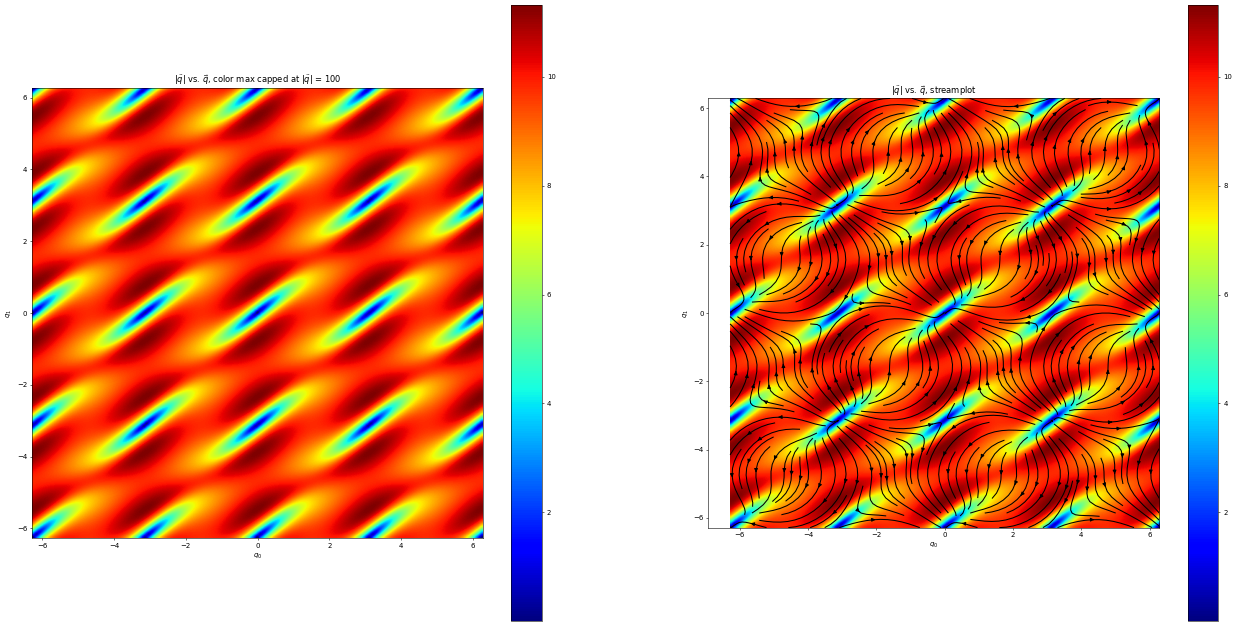
\includegraphics[scale=0.22]{accelerations_zv_true.png}
	\label{fig:accelerations_zv_true}
\end{figure}

After several hours of training, the model results (for the zero-velocity slice)  match the true results relatively well:

\begin{figure}[H]
	\caption{Model acceleration vs. position, zero velocity}
	\centering
	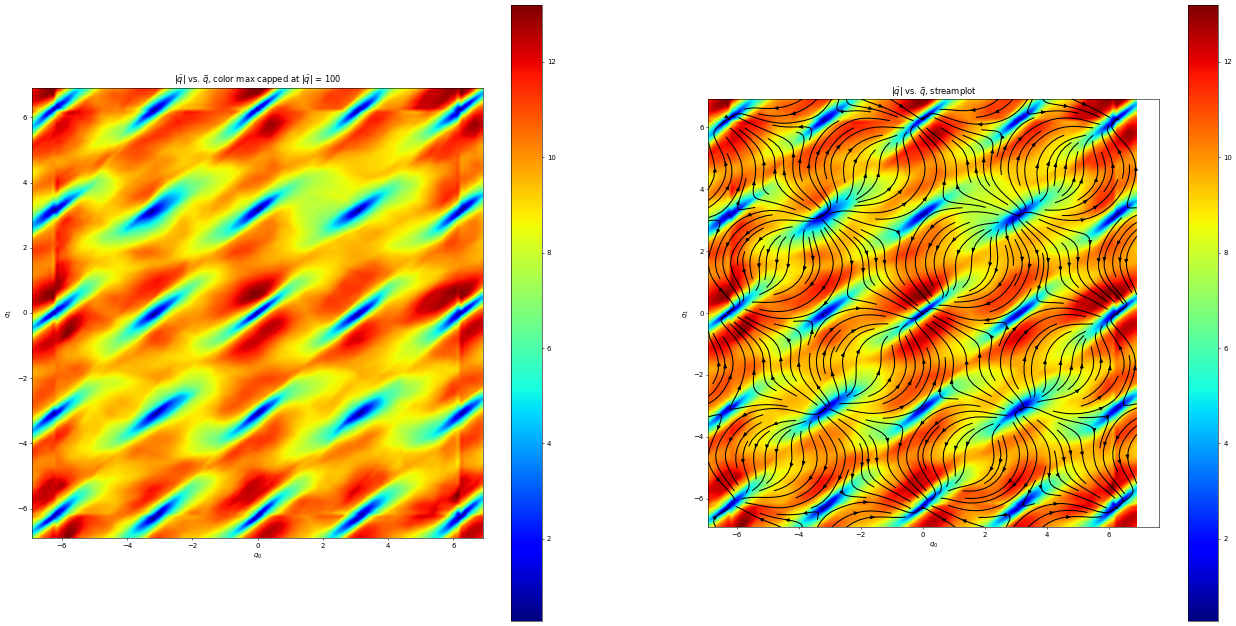
\includegraphics[scale=0.22]{accelerations_zv_model.png}
	\label{fig:accelerations_zv_model}
\end{figure}

The double pendulum equilibria (zero acceleration) at $q = 0 \mod{pi}$ are all present and well-defined, and the areas immediately surrounding each equilibrium show the correct stream behavior. Howeever, some of the intermediate areas are not well-respresented by the model and carry a deformation from the true system.

Now plotting the magnitude of the error in acceleration, we see that the model generally fits quite well but has a couple of regions with large error. Additionally, the boundary between one domain (e.g. $\{q\in(-2\pi,2\pi)\}$ $\to$ $\{q\in(2\pi,4\pi))\}$ shows a discontinuty coming from taking the positions mod $2\pi$.

\begin{figure}[H]
	\caption{Model acceleration vs. position, zero velocity}
	\centering
	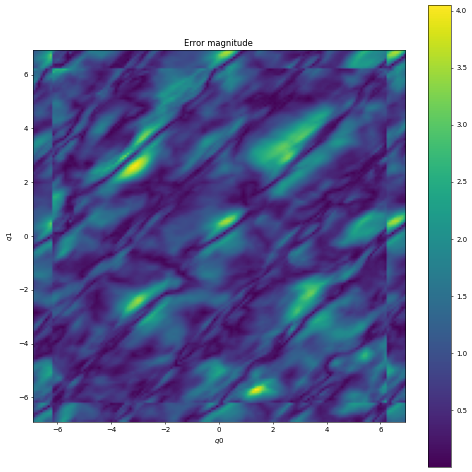
\includegraphics[scale=0.30]{acceleration_model_error.png}
	\label{fig:acceleration_model_error}
\end{figure}



While animating the results, I noticed that the resulting model trajectories often develop a position offset relative to the true trajectories, but tend to match qualtitative behavior (spinning quickly, looping, transferring energy from one pendulum to the other, etc.) at the same time as the true system.



\newpage
\begin{appendices}
\section{Bibliography}
\printbibliography
\end{appendices}

\end{document}